\subsection{Pneumatikzylinder}

\begin{tabular}{p{3.6cm}p{9.4cm}}
\textit{Typ}              & Ballmaschine \\ 
\textit{Datum}:           & 08.10.2014   \\
\textit{Ort}:             & Bachmann Engineering AG (Zofingen) \\
\textit{Tester}:          & Gruppe 32\\
\textit{Ziel des Testes}: & Der gebaute Prototyp wird auf die Wurfwiederholgenauigkeit getestet. \\
\textit{Fazit / Verbesserungs-\newline vorschlag}: & Ein Pneumatikzylinder arbeitet sehr zielgenau und schnell. Falls dieses Verfahren in die engere Auswahl kommt, müssen die Parameter wie Beschleunigung, Abschussgeschwindigkeit und Druck berechnet werden.\\ 
\textit{Ziel erreicht}:& Ja\\
\end{tabular}

\begin{figure}[h!]
	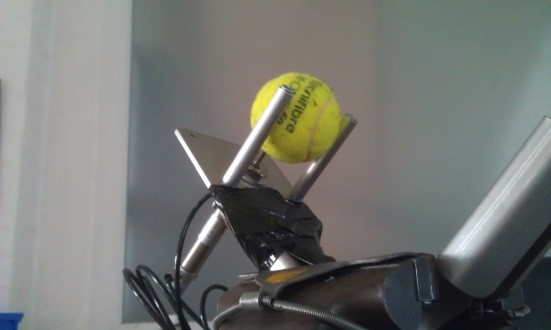
\includegraphics[width=5cm]{Funktionstests/Bilder/PneumatikzylinderBild.jpg}
	\centering
	\caption{Funktionsmuster Pneumatikzylinder} 
\label{abb:PneumatikzylinderBild}
\end{figure}